\chapter{Evaluation}

\begin{figure}
    \centering
    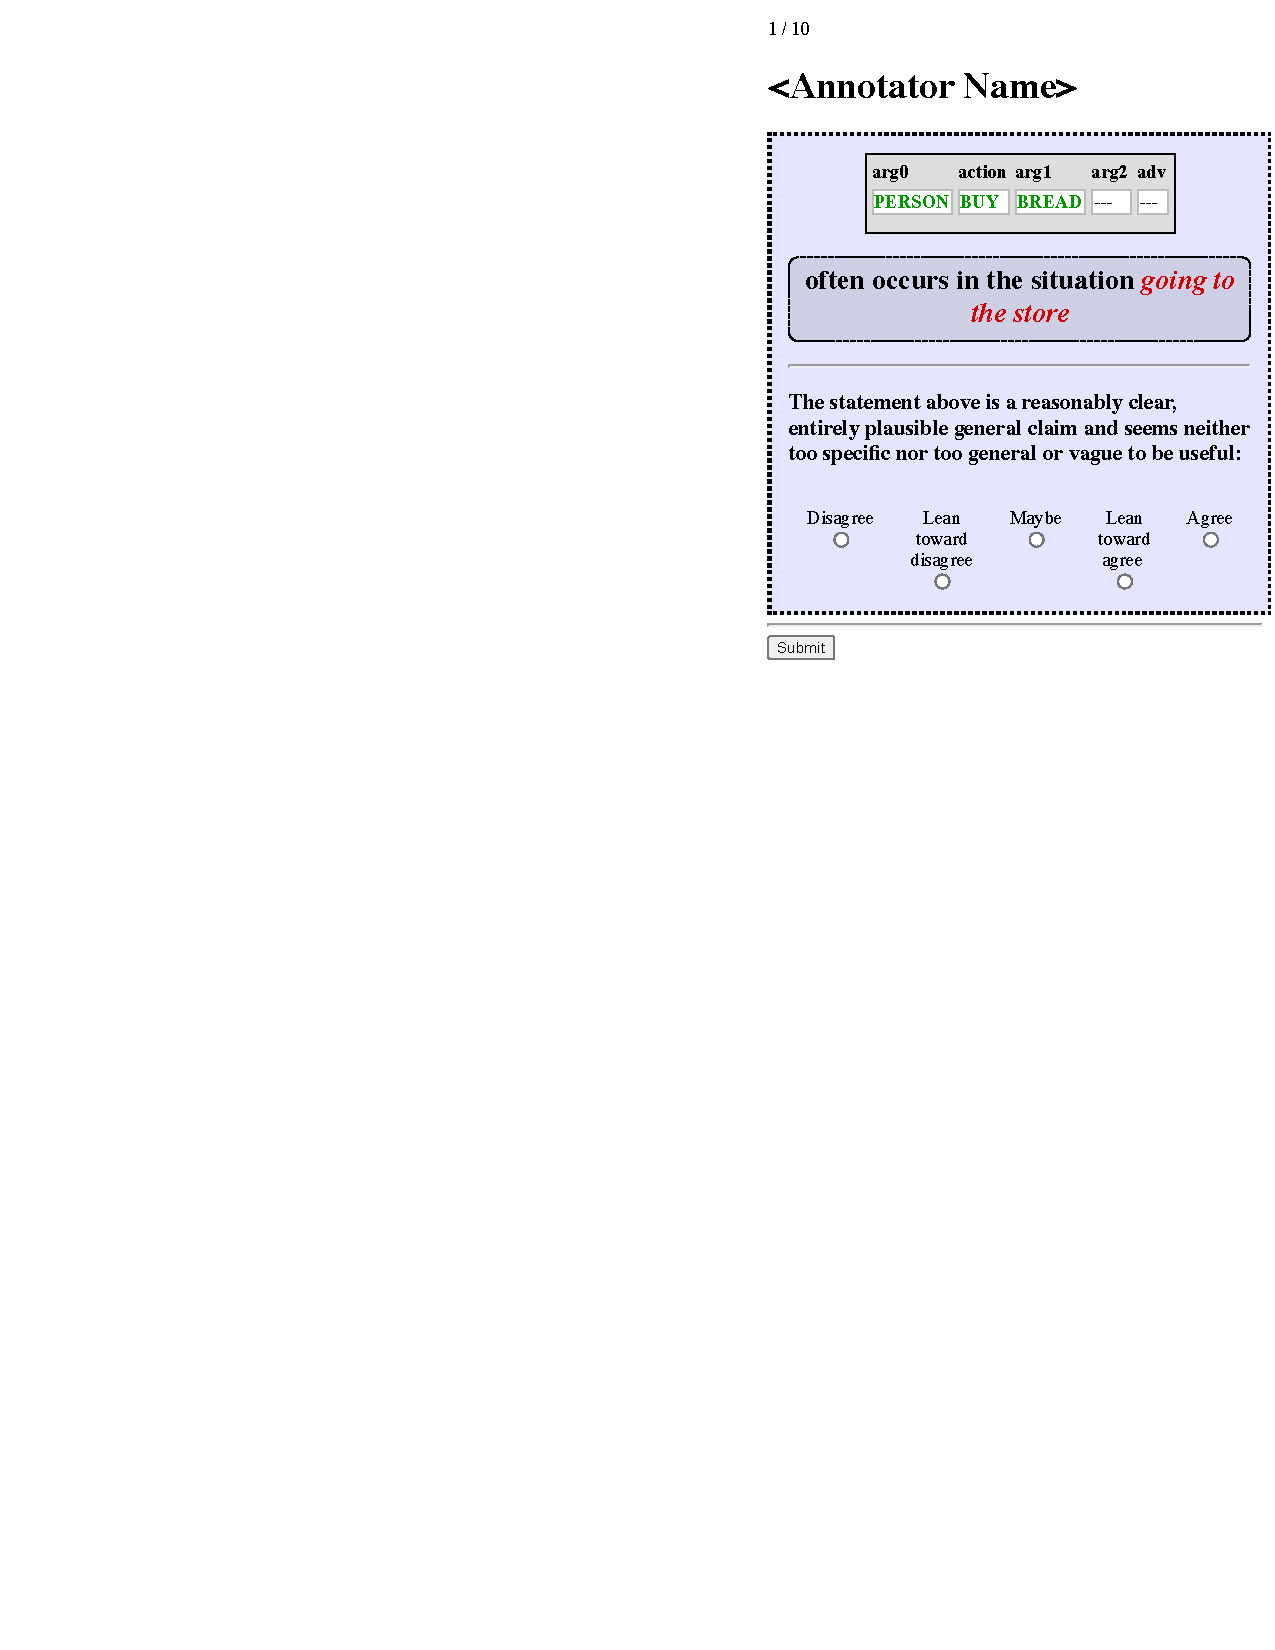
\includegraphics[width=0.5\textwidth]{CH4_learning/evaleg3.pdf}
    \caption{An example of a form presented to a schema quality evaluator for a \textit{step} formula.}
    \label{fig:step_eval_eg}
\end{figure}

\begin{figure}
    \centering
    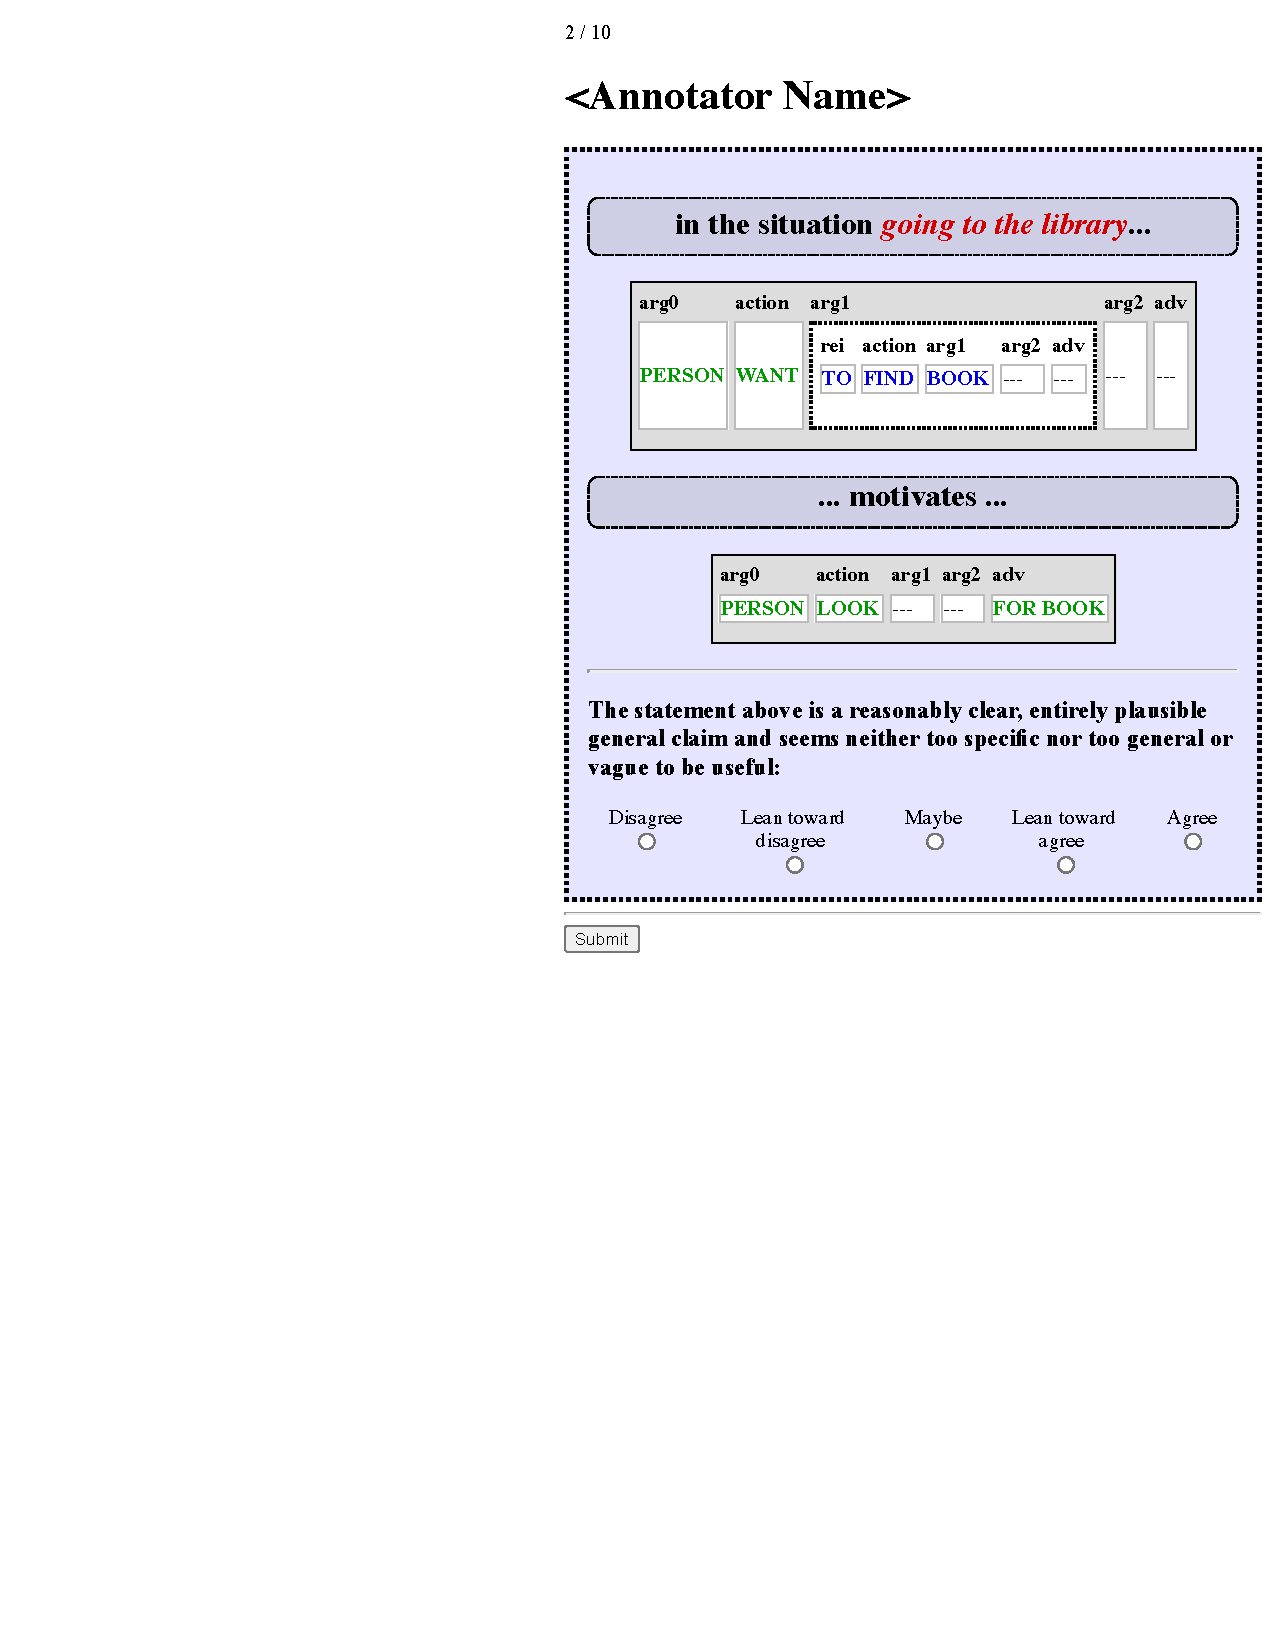
\includegraphics[width=0.5\textwidth]{CH4_learning/evaleg4.pdf}
    \caption{An example of a form presented to a schema quality evaluator for a \textit{goal} formula.}
    \label{fig:goal_eval_eg}
\end{figure}

EL schemas enable consistent, structured, and interpretable inferences about novel text, by matching pieces of the text to pieces of the schema, replacing schema variables with entities from the story, and treating other formulas in the schema that use those newly-filled variables as inferences. Here, we describe an assessment of the generality and relevance of the schema formulas learned by NESL.
%In addition to inferences, we would like to evaluate whether the schemas we obtain are both \textit{topically cohesive}, i.e., focused descriptions of one kind of situation; and \textit{interesting}, i.e., capable of generating useful and novel inferences about situations, rather than obvious or redundant ones.